\lezione{Lezione 15}{18/11/2024}
Calcoliamo ora la trasformata del \textit{pettine di impulsi} $\delta_{T_S}$:
\begin{align*}
    \Delta_{T_S}(f) &= \fourier\{\frac{1}{T_S}\sum_{n = -\infty}^{+\infty} e^{j2\pi\frac{n}{Ts}t}\} =\\
                    &= \frac{1}{T_S}\sum_{n = -\infty}^{+\infty}\fourier \{  e^{j2\pi\frac{n}{Ts}t}\}=\\
                    &= \frac{1}{T_S}\sum_{n = -\infty}^{+\infty} \delta\left(f - \frac{n}{Ts}\right)
\end{align*}
Possiamo dunque notare quest'importante coppia di Fourier:
\begin{equation}
    \underbrace{\sum_{-\infty}^{+\infty} \delta (t - nT_S)}_{\delta_{T_S}(t)} \fCouple \underbrace{\frac{1}{T_S}\sum_{n = -\infty}^{+\infty} \delta\left(f - \frac{n}{Ts}\right)}_{\Delta_{T_S}(f)}
\end{equation}
Da ciò possiamo notare come una serie di impulsi nei tempi corrisponde ad una serie di impulsi nelle frequenze.

\paragraph{Spettro del Campionamento.}Da ciò possiamo dunque ricavarci lo spettro del segnale campionato:
\begin{align*}
    S_C(f) &= S(f) \ast \Delta_{T_S}(f) =\\
           &= S(f) \ast \{ \frac{1}{T_S} \sum_{n = -\infty}^{+\infty} \delta\left(f - \frac{n}{Ts}\right)\}=\\
           &= \frac{1}{T_S} \sum_{n = -\infty}^{+\infty}\{  S(f) \ast  \delta\left(f - \frac{n}{Ts}\right)\}=\\
           &= \frac{1}{T_S} \sum_{n = -\infty}^{+\infty}  S\left(f - \frac{n}{Ts}\right)
\end{align*}
Cioè, campionando un segnale con periodo $T_S$, nel dominio delle frequenze lo spettro ottenuto è uguale a \textbf{infinite repliche del segnale di partenza}, ognuna delle quali
centrata in $n/T_S$.\\
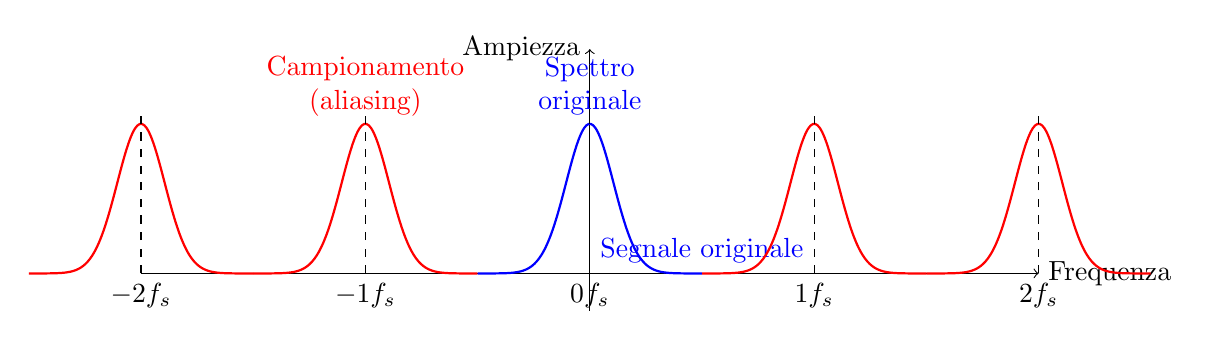
\begin{tikzpicture}[scale=0.95]

    % Assi
    \draw[->] (-6,0) -- (6,0) node[right] {Frequenza};
    \draw[->] (0,-0.5) -- (0,3) node[left] {Ampiezza};
    
    % Spettro del segnale originale
    \draw[thick,blue,smooth] plot[domain=-1.5:1.5,samples=100] (\x,{2*exp(-5*(\x)^2)}) node[above] {Segnale originale};
    
    % Spettri ripetuti (campionamento)
    \foreach \k in {-2,-1,1,2} {
        \draw[thick,red,smooth] plot[domain=-1.5:1.5,samples=100] 
            ({\x + \k*3},{2*exp(-5*(\x)^2)});
    }
    
    % Annotazioni
    \foreach \k in {-2,-1,0,1,2} {
        \draw[dashed] ({\k*3},0) -- ({\k*3},2.2);
        \node[below] at ({\k*3},0) {\(\k f_s\)};
    }
    
    % Etichetta
    \node at (-3,2.5) [align=center,red] {Campionamento \\ (aliasing)};
    \node at (0,2.5) [align=center,blue] {Spettro \\ originale};
    
    \end{tikzpicture}

\paragraph{Repliche Disgiunte e Sovrapposte.}Consideriamo ora i 2 possibili casi:
\begin{itemize}
    \item $W < f_S/2$ (dove $W$ è la banda del segnale, $f_S$ è la frequenza di campionamento): otteniamo repliche disgiunte come nel grafico soprastante
    \item $W > f_S/2$ : otteniamo repliche che si sovrappongono in parte
\end{itemize}
Questa distinzione è importante perchè quando facciamo operazione di filtraggio del segnale e con un filtro passa-basso selezioniamo
solo una di queste repliche, possiamo ottenere il segnale di partenza.\\
\bigskip
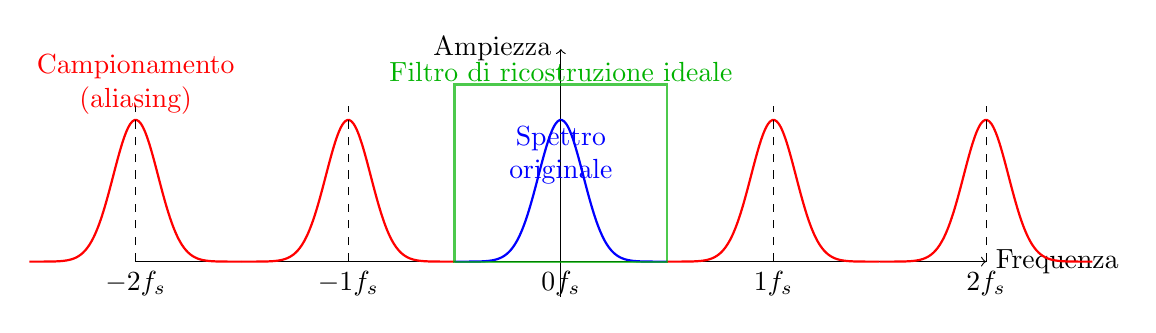
\begin{tikzpicture}[scale=0.9]

    % Assi
    \draw[->] (-6,0) -- (6,0) node[right] {Frequenza};
    \draw[->] (0,-0.5) -- (0,3) node[left] {Ampiezza};
    
    % Spettro del segnale originale
    \draw[thick,blue,smooth] plot[domain=-1.5:1.5,samples=100] (\x,{2*exp(-5*(\x)^2)});
    
    % Spettri ripetuti (campionamento)
    \foreach \k in {-2,-1,1,2} {
        \draw[thick,red,smooth] plot[domain=-1.5:1.5,samples=100] 
            ({\x + \k*3},{2*exp(-5*(\x)^2)});
    }
    
    % Annotazioni per i multipli di fs
    \foreach \k in {-2,-1,0,1,2} {
        \draw[dashed] ({\k*3},0) -- ({\k*3},2.2);
        \node[below] at ({\k*3},0) {\(\k f_s\)};
    }
    
    % Filtro di ricostruzione ideale
    \draw[thick,green!70!black,opacity=0.7] 
        plot[domain=-1.5:1.5,samples=100] (\x,{2.5}) -- (1.5,2.5) -- (1.5,0) -- (-1.5,0) -- (-1.5,2.5) -- cycle;
    \node[above,green!70!black] at (0,2.4) {Filtro di ricostruzione ideale};
    
    % Etichette
    \node at (-6,2.5) [align=center,red] {Campionamento \\ (aliasing)};
    \node at (0,1.5) [align=center,blue] {Spettro \\ originale};
    
    \end{tikzpicture}
\subsection{Teorema di Nyquist-Shannon}
\textit{Un segnale con banda limitata $W$ superiormente può essere ricostruito univocamente a partire dai suoi campioni se e solo se
 il campionamento avviene a frequenza maggiore di $2W$}, ossia:
 \begin{equation}
    f_S > 2W
 \end{equation}

\subsection{Ricostruzione nel dominio delle frequenze}
Usando il filtro passa-basso come avevo mostrato prima con $f_T = f_S/2 = f_N$ con $f_N$ la \textit{frequenza di Nyquist},
possiamo ricostruire il segnale di partenza. Consideriamo il filtro:
\begin{equation}
    H_R(f) = \begin{cases}
        T_S & |f| \leq f_N\\
        0   & \text{altrimenti}
    \end{cases}= T_S\text{rect}\left(\frac{f}{f_S}\right)
\end{equation}
Allora:
\begin{align*}
    S_C(f)H_R(f) &= \frac{1}{T_S} \sum_{n = -\infty}^{+\infty} s\left(f - \frac{n}{T_S}\right) \cdot T_S \text{rect}\left(\frac{f}{f_S}\right) =\\
                 &= \cancel{\frac{1}{T_S}} \sum_{n = -\infty}^{+\infty} s\left(f - \frac{n}{T_S}\right) \cdot \cancel{T_S} \text{rect}(fT_S) =\\
                 &= \sum_{n = -\infty}^{+\infty} s\left(f - \frac{n}{T_S}\right) \cdot \text{rect}(fT_S) =\\
                 &= S(f)
\end{align*}
Riottenendo dunque $S(f)$, possiamo definire $H_R(f)$ come il \textbf{filtro di ricostruzione ideale}

\subsection{Ricostruzione nel dominio dei tempi}
Per calcolare $s(t)$ basta antitrasformare quanto calcolato prima:
\begin{equation}
    S(f) = S_C(f)H_R(f) \fAnticouple  s_C(t) \ast h_R(t)
\end{equation}
Dalle coppie notevoli, ci accorgiamo che $h_R(t) = \text{sinc}\left(\frac{t}{T_S}\right)$, ossia la risposta all'impulso è un 
seno cardinale che si annulla in tutti i punti in cui abbiamo campionato, tranne che in 0, o meglio:
\begin{equation}
    h_R(nT_S) = \begin{cases}
        1 & \text{ se } n = 0\\
        0 & \text{ se } n \neq 0
    \end{cases}
\end{equation}\\
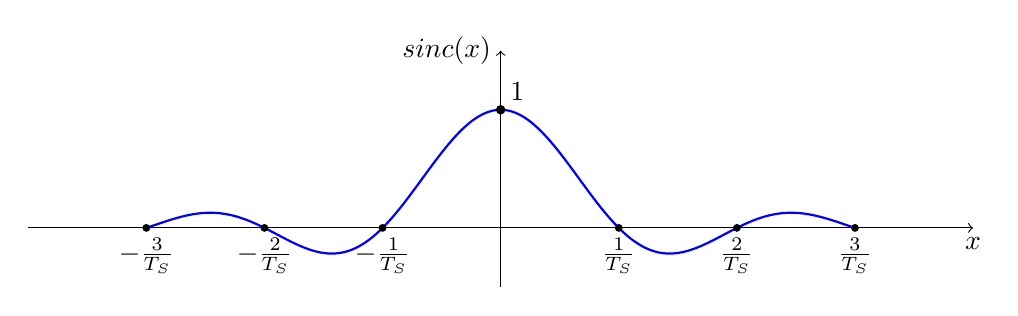
\begin{tikzpicture}[scale=1.5]

    % Assi
    \draw[->] (-4,0) -- (4,0) node[below] {$x$};
    \draw[->] (0,-0.5) -- (0,1.5) node[left] {$\text{sinc}(x)$};
    
    % Disegno della funzione sinc
    \draw[thick,blue,smooth,domain=-3:3,samples=400] 
        plot (\x,{(sin(180*\x)/(\x*pi))});
    
    % Punto centrale
    \filldraw (0,1) circle (1pt) node[above right] {$1$};
    
    \foreach \k in {-3,-2,...,3} {
        \ifnum\k=0
        \else
            \filldraw (\k,0) circle (0.8pt);
        \fi
    }
    
    % Etichette per i zeri
    \node[below] at (-3,0) {$-\frac{3}{T_S}$};
    \node[below] at (-2,0) {$-\frac{2}{T_S}$};
    \node[below] at (-1,0) {$-\frac{1}{T_S}$};
    \node[below] at (1,0) {$\frac{1}{T_S}$};
    \node[below] at (2,0) {$\frac{2}{T_S}$};
    \node[below] at (3,0) {$\frac{3}{T_S}$};
    
    \end{tikzpicture}

Calcoliamo ora $s(t)$:
\begin{align*}
    s(t) &= s_C(t) \ast h_R(t) = \\
         &= \left\{ \sum_{-\infty}^{+\infty} s(nT_S) \delta(t - nT_S)\right\} \ast \text{sinc}\left(\frac{t}{T_S}\right) = \\
         &= \sum_{-\infty}^{+\infty} s(nT_S)\left\{  \delta(t - nT_S) \ast \text{sinc}\left(\frac{t}{T_S}\right)\right\} = \\ 
         &= \sum_{-\infty}^{+\infty} s(nT_S) \text{sinc}\left(\frac{t - nT_S}{T_S}\right) \tag{per \eqref{prop: ConvDelta}}
\end{align*}
Cioè il segnale ricostruito è dato dalla combinazione lineari di tanti seni cardinali.

\subsection{Aliasing}
Nel caso in cui avessimo campionato il segnale con frequenza di campionamento $f_S < f_N$ si verifica questa situazione:\\
\begin{center}
    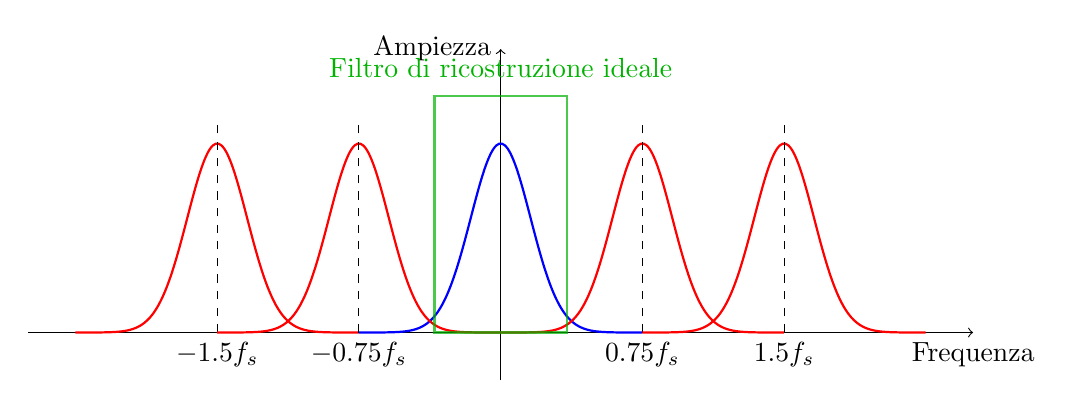
\begin{tikzpicture}[scale=1.2]

        % Assi
        \draw[->] (-5,0) -- (5,0) node[below] {Frequenza};
        \draw[->] (0,-0.5) -- (0,3) node[left] {Ampiezza};
        
        % Spettro del segnale originale
        \draw[thick,blue,smooth] plot[domain=-1.5:1.5,samples=100] (\x,{2*exp(-5*(\x)^2)});
        
        % Spettri ripetuti (campionamento sottocampionamento)
        \foreach \k in {-1.5,-0.75,0.75,1.5} {
            \draw[thick,red,smooth] plot[domain=-1.5:1.5,samples=100] 
                ({\x + \k*2},{2*exp(-5*(\x)^2)});
            \draw[dashed] ({\k*2},0) -- ({\k*2},2.2);
            \node[below] at ({\k*2},0) {\(\k f_s\)};
        }
        
        % Filtro di ricostruzione ideale
            \draw[thick,green!70!black,opacity=0.7] 
            plot[domain=-0.7:0.7,samples=100] (\x,{2.5}) -- (0.7,2.5) -- (0.7,0) -- (-0.7,0) -- (-0.7,2.5) -- cycle;
            \node[above,green!70!black] at (0,2.6) {Filtro di ricostruzione ideale};
        
        \end{tikzpicture}
\end{center}
Dal grafico è possibile notare come le \textit{frequenze illegali} che appartengono alla banda ma non vengono selezionate dal filtro,
finiscono per essere sostituite dalla loro versione specchiata, cioè un'altra nota con lo stesso contributo. Per cui il suono si altera
e perdiamo qualità. Questo effetto è detto \textbf{Aliasing} o Equivocazione.
Per evitare questo effetto, spesso si effettua preprocessing sul segnale per \textit{adattare} il segnale al campionamento che subirà successivamente
tagliando le opportune frequenze. Questi filtri che svolgono ciò vengono detti \textbf{Anti-Aliasing}.